\documentclass[../main/main.tex]{subfiles}

\newdate{date}{11}{11}{2020}


\begin{document}

\marginpar{ \textbf{Laboratory 16.} \\  \displaydate{date}. \\ Compiled:  \today.}

\section{Correzioni circuito amplificatore}

Le scorse volte invertivamo i pin \( V_{in+} \) e \( V_{in-} \). Abbiamo corretto tutto. In Fig. \ref{fig:16_1} si ritrova in alto a sinistra il circuito dell'amplificatore, in basso lo schema del modulo NIM corretto e in alto a destra lo schema del cablaggio corretto.

\begin{figure}[h!]
\begin{minipage}[c]{0.5\linewidth}
\centering
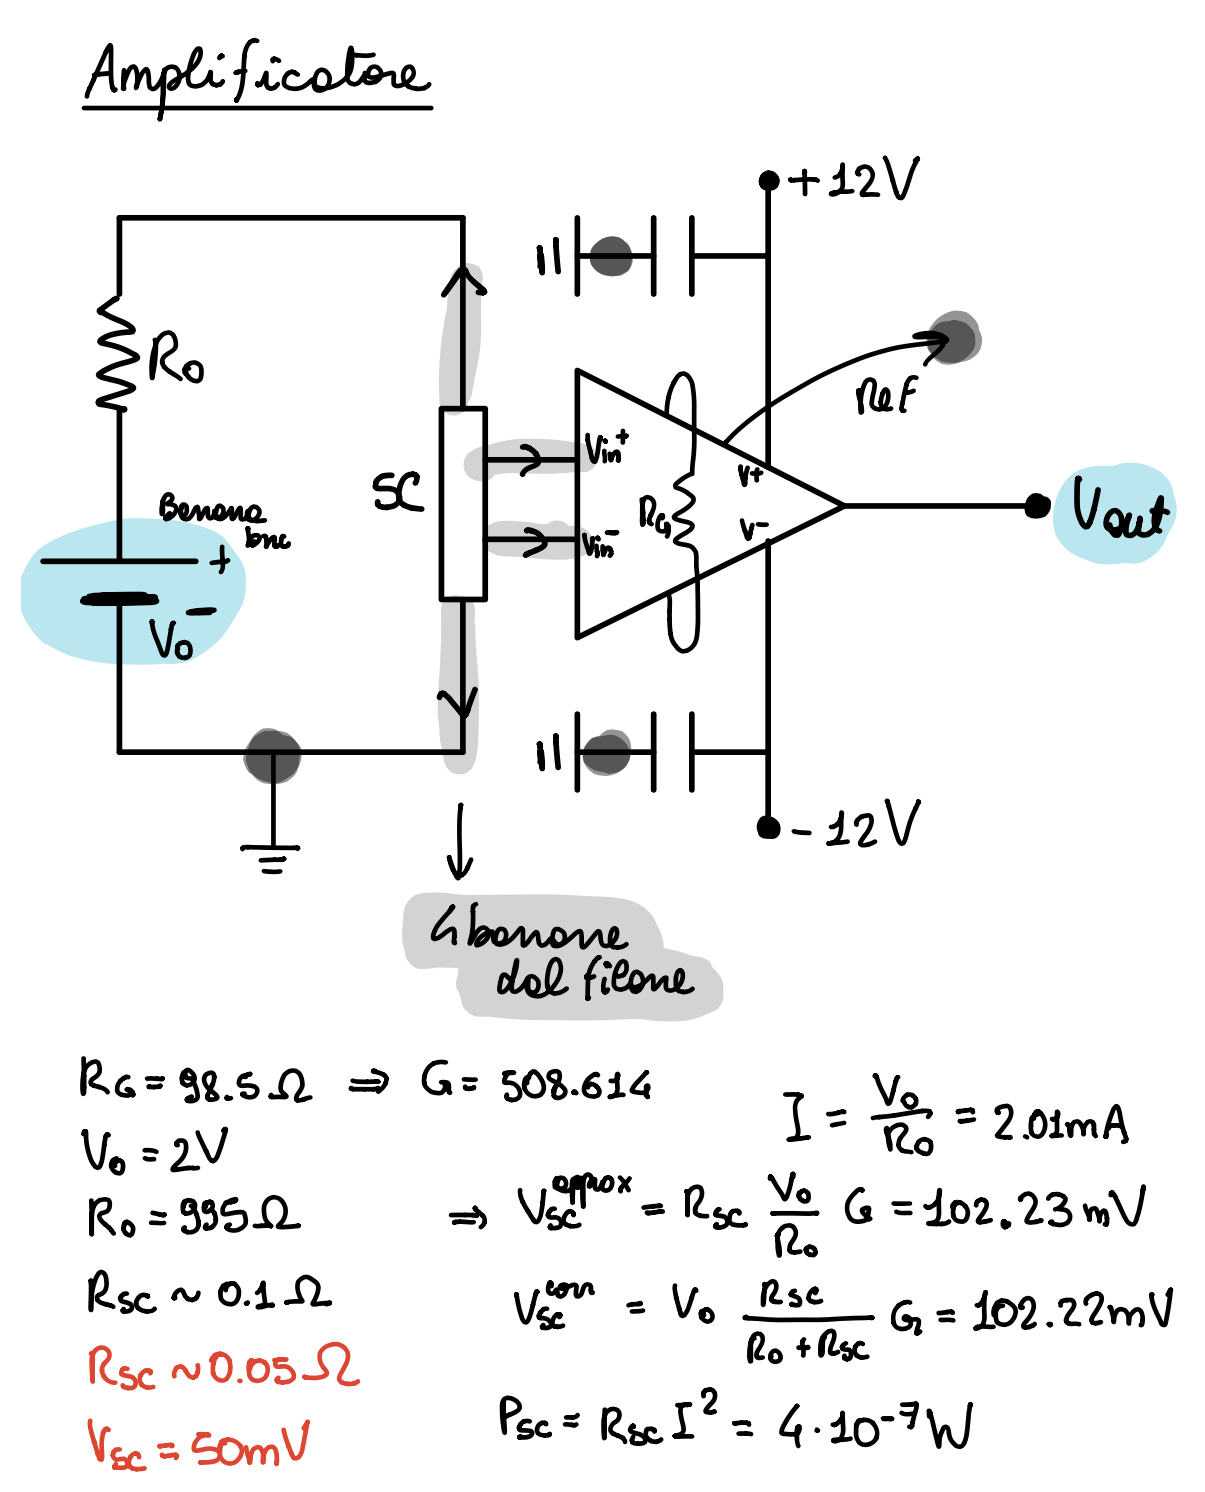
\includegraphics[width=1\textwidth]{../lessons/image/16/amplificatore.png}
\end{minipage}
\begin{minipage}[]{0.5\linewidth}
\centering
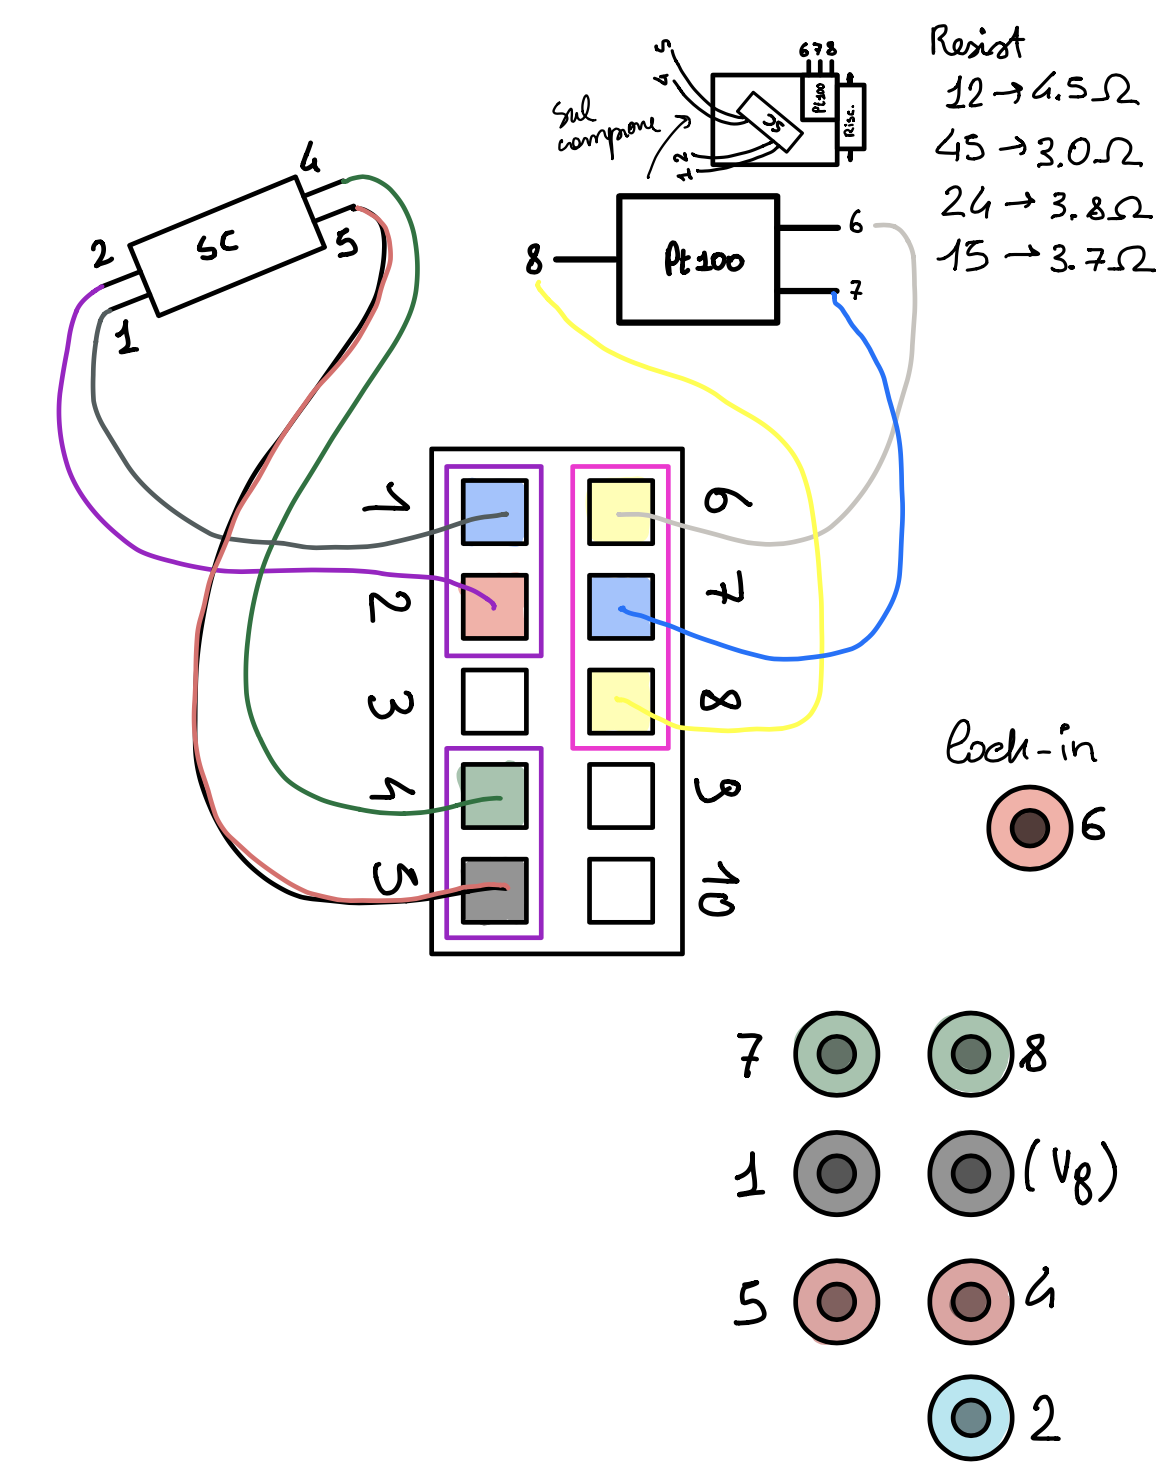
\includegraphics[width=1\textwidth]{../lessons/image/16/cablaggio.png}
\end{minipage}
\vspace{1cm}
\begin{minipage}[]{1\linewidth}
\centering
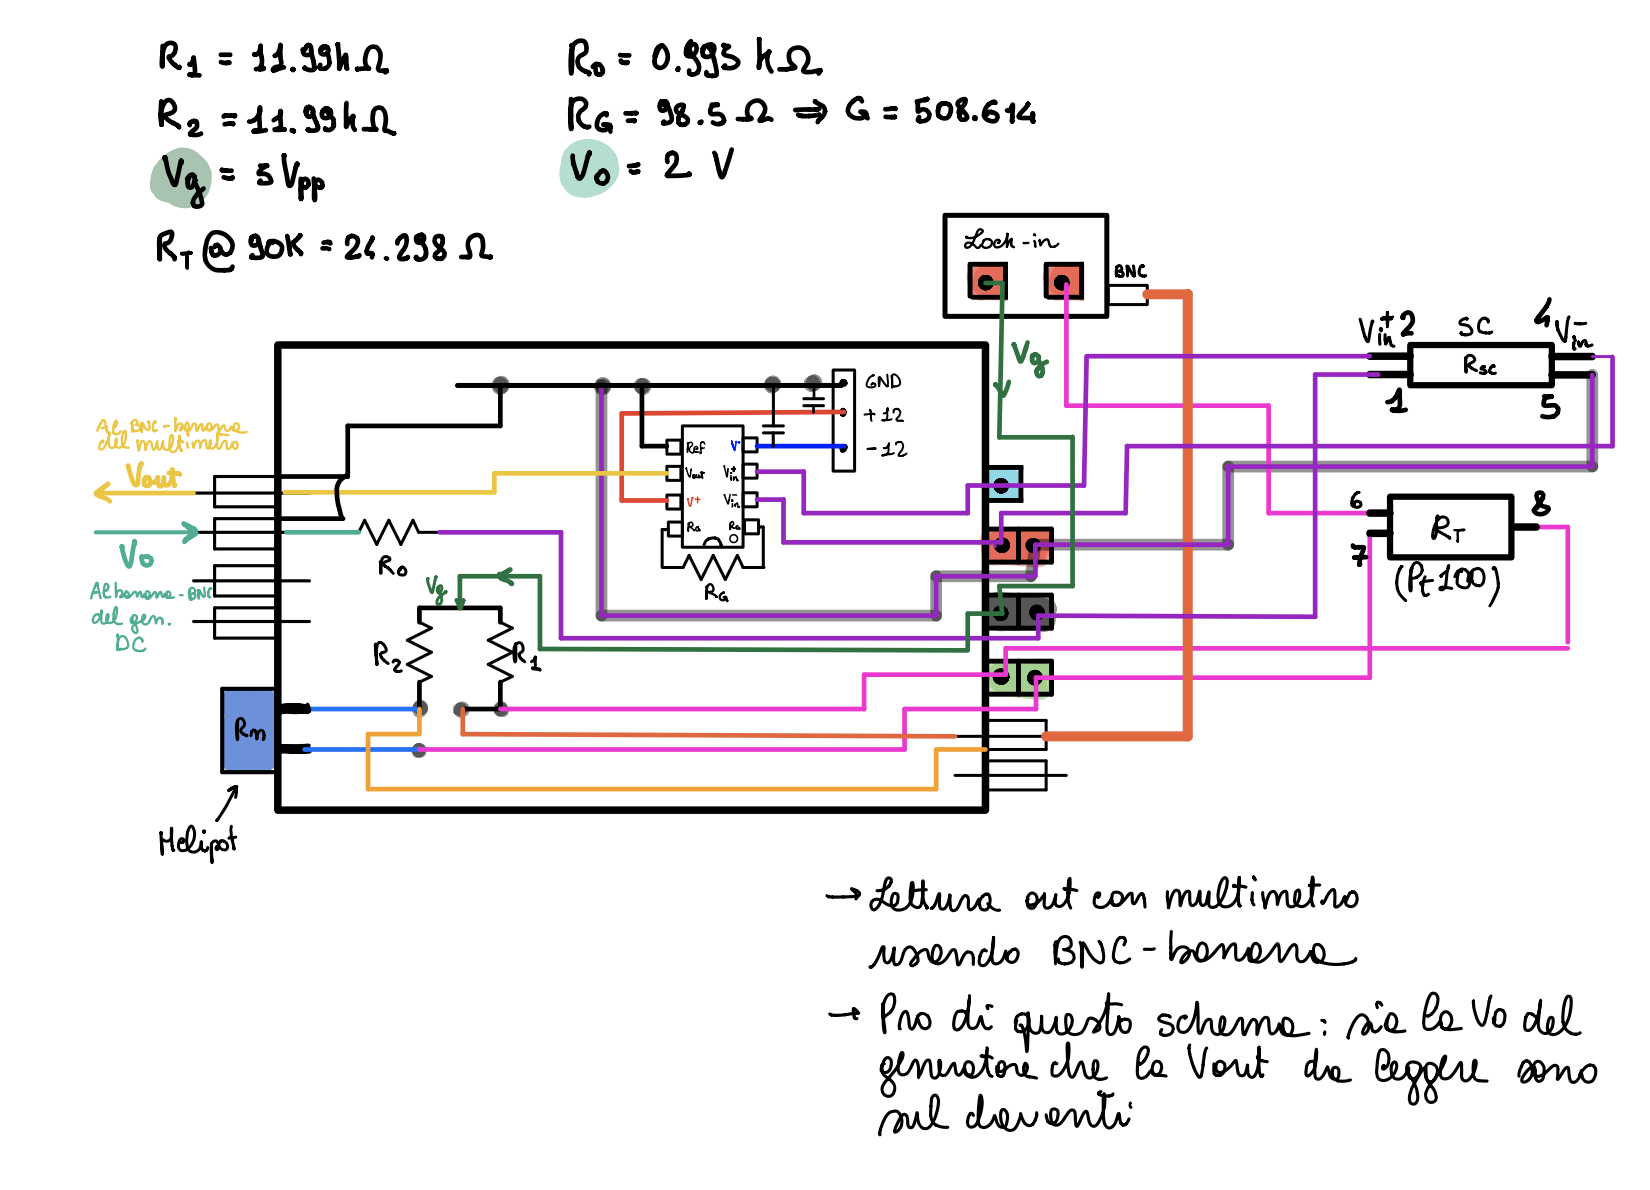
\includegraphics[width=1\textwidth]{../lessons/image/16/nim.png}
\end{minipage}
\caption{\label{fig:16_1} Schemi definitivi prima dell'acquisizione delle misure. In alto a sinistra schema amplificatore. In alto a destra schema cablaggio fili. In basso schema modulo NIM.}
\end{figure}

In particolare, i cavi nel retro del modulo NIM sono collegati come in Fig. \ref{fig:16_2}.

\begin{figure}[h!]
\centering
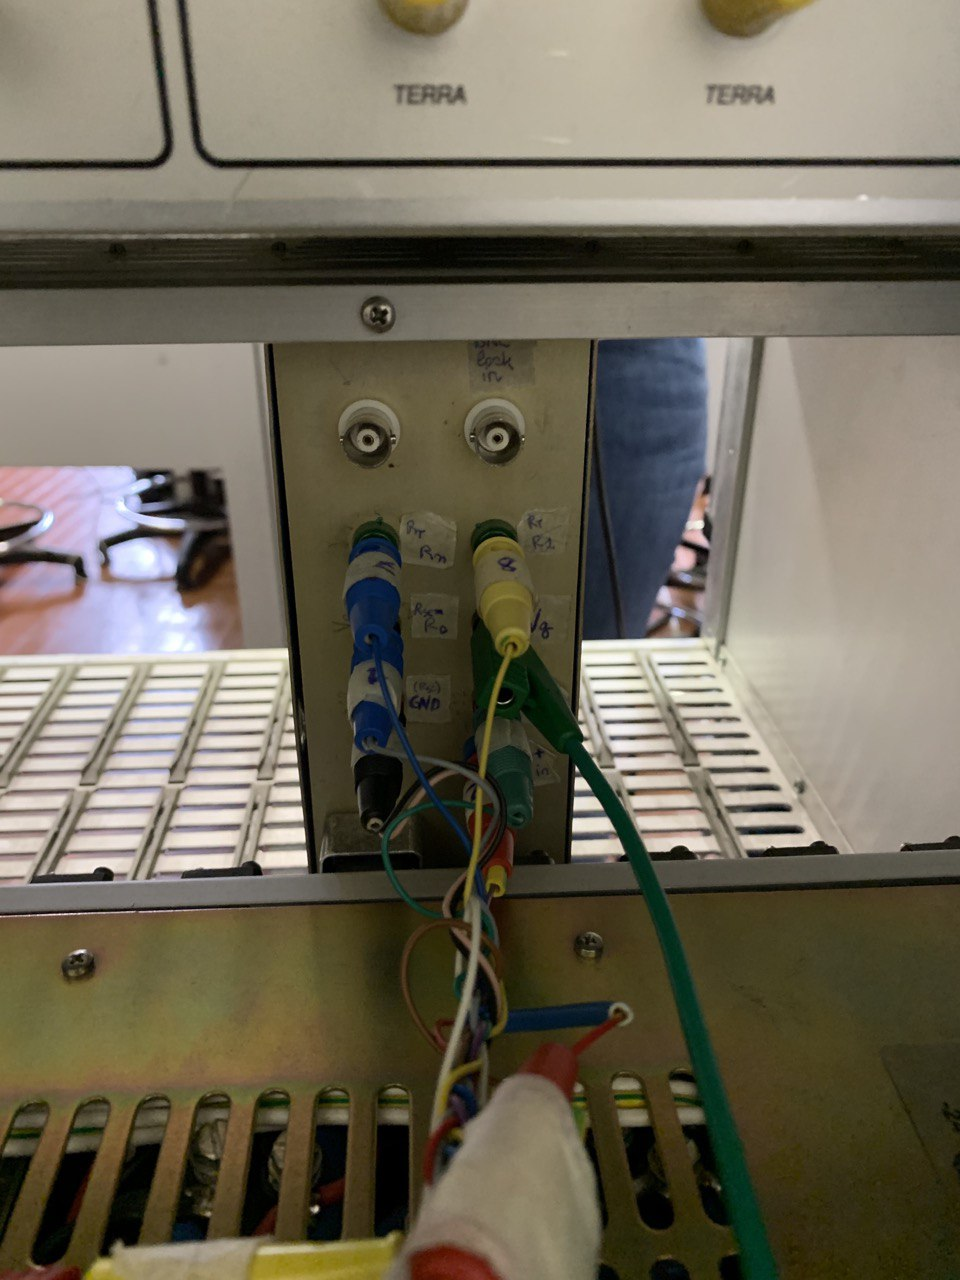
\includegraphics[width=0.6\textwidth]{../lessons/image/16/retro_nim.jpg}
\caption{\label{fig:16_2} Collegamento cavi nel retro del modulo NIM.}
\end{figure}


\section{Finalmente: misure}
Abbiamo collegato l'arduino per effettuare le misure.
\begin{itemize}
\item abbiamo collegato l'output del termometro del dito freddo e abbiamo impostato come resistenza dei fili 6.5;
\item abbiamo collegato l'output dell'amplificatore \( V_{out} \).
\end{itemize}
Notiamo come al diminuire della temperatura, \( V_{out} \) aumenti sempre di più. Il problema può essere un potenziale di contatto che si crea (che dipende dalla temperatura). Infatti, si può creare una forza elettromotrice indotta che aumenta l'offset.

Oggi abbiamo effettuato un primo test di misure in cui abbiamo raffreddato e riscaldato il campione varie volte. Abbiamo inoltre cambiato più volte il potenziale \( V_0 \) dato in input per poter visualizzare salti maggiori. Abbiamo osservato che il campione transice ad una resistenza di \( R_v \sim 32 \Omega \) che corrisponde ad una temperatura di circa \( 110  \) K.







\end{document}
